\secnumbersection{Desarrollo previo}
\hlabel{sec:3}

\subsection{COMPARATIVA TÉCNICA ENTRE TARJETAS GRÁFICAS.}

\hlabel{sec:3.1}

Para la experimentación realizada en las siguientes secciones de esta memoria, se utilizaron dos tarjetas gráficas, de NVIDIA y AMD respectivamente, que tienen especificaciones similares en termino de la gama a la que pertenecen respecto a su año de salida. 
Tomando lo anterior en cuenta, y debido al desabastecimiento general de tarjetas gráficas que ha sufrido el mercado tecnológico en los últimos años es que se escogió la GPU NVIDIA GTX 960M de arquitectura código Maxwell y AMD RX570 de arquitectura código Polaris.
Cabe destacar que la tarjeta GTX 960M estuvo enfocada en la venta de laptops de alto rendimiento~\cite{gtx960m} mientras que la tarjeta RX570 está pensada para computadoras personales de escritorio, ambas como partes de una gama media-alta en el mercado.

Como se mencionó anteriormente la GPU GeForce GTX 960M, lanzada al mercado el año 2015, corresponde a la a la primera generación de la arquitectura Maxwell, pues hace uso de un chip GM107.
Este chip esta compuesto por un Clúster de Proceso Gráfico (GPC, del ingles \textit{Graphic Processing Cluster}), dos controladores de memoria encargados del flujo de memoria entre CPU y GPU, 2 \textit{Megabyte} de memoria caché L2 y 16 Unidades de Salida de Renderizado (ROP), las cuales tienen como aplicación generar cálculos finales en el renderizado necesario para los programas que hagan uso de la GPU.
A su vez, el GPC está compuesto por 5 Multiprocesadores de Streaming (SM, del inglés \textit{Streaming Multiprocessor}) los cuales se conforman cada uno por un motor de Polimorfismo (del inglés \textit{Polymorph engine}) encargado de gestionar los recursos para el renderizado general, 8 motores de textura encargados del mapeo textura-modelo, \textit{Warp Schedulers} y núcleos CUDA (CU).
En esta arquitectura, la unidad básica de procesamiento corresponde al núcleo CUDA, y la unidad mínima de ejecución corresponde al \textit{Warp}.
En general, las tarjetas NVIDIA actuales consideran un \textit{Warp} como 32 hilos de ejecución, y en general la arquitectura Maxwell tiene la capacidad de enviar a cada núcleo 2 instrucciones por cada \textit{clock} de la tarjeta \cite{nwhitepaper}.
Una representación aproximada de los componentes listados se puede observar en la Figura~\ref{fig:6}.


\begin{figure}[h!]
    \centering
    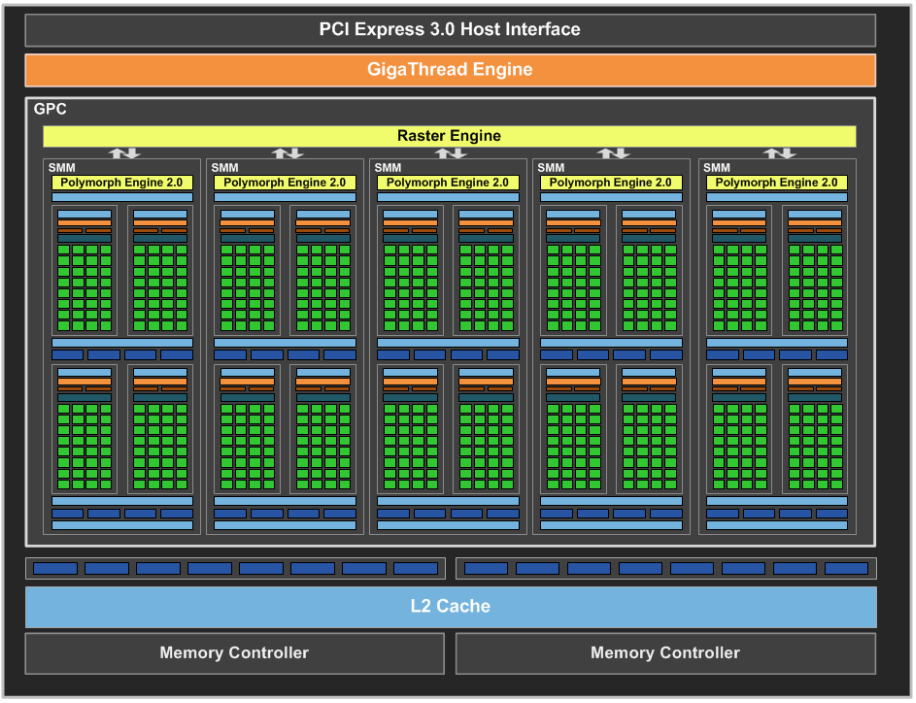
\includegraphics[width=.8\textwidth]{Figures/nvidia.png}
    \caption{Diagrama de bloque sobre arquitectura de chip GM107}
    \label{fig:6}
\end{figure}


Por otro lado, la GPU RX570 fue lanzada al mercado el año 2017 y corresponde a la arquitectura Polaris al usar un chip Polaris 20XL. 
La estructura general de esta arquitectura esta compuesta por un Procesador de Comandos Gráficos (del inglés, \textit{Graphics Command Processor}), distintos Motores de Computo Asíncrono (del inglés, \textit{Asynchronous Compute Engine }) y \textit{Hardware Scheduler} encargados de la gestión y ejecución asíncrona de ciertas llamadas a la GPU, y por último el conjunto de memoria L2 (de 2 \textit{Megabyte} para la tarjeta usada).
De la misma forma que el GPC en la tarjeta de NVIDIA, el Procesador de Comandos Gráficos se divide varios Motores de Sombreado (del inglés, \textit{Shader Engines}), que a su vez se dividen en distintas sub unidades, de las cuales destacan Procesadores Geométricos encargados del renderizado gráfico, y Unidades de Computo (del inglés, \textit{Compute Units}) las cuales corresponden a un conjunto de \textit{ROP's}, motores de textura y Procesadores de Sombreado (del inglés, \textit{Shader Processor}) \cite{awhitepaper}.
En la arquitectura Polaris, la unidad básica de procesamiento corresponde al \textit{Shader Processor}, y la unidad mínima de ejecución corresponde al \textit{Wavefront}.
Por definición, 16 \textit{Wavefronts} corresponden a un \textit{Workgroup} y cada \textit{Wavefront} esta conformado por 64 hilos de ejecución.
La Figura~\ref{fig:7} presenta una representación de la arquitectura y sus componentes listados.

\begin{figure}[h!]
    \centering
    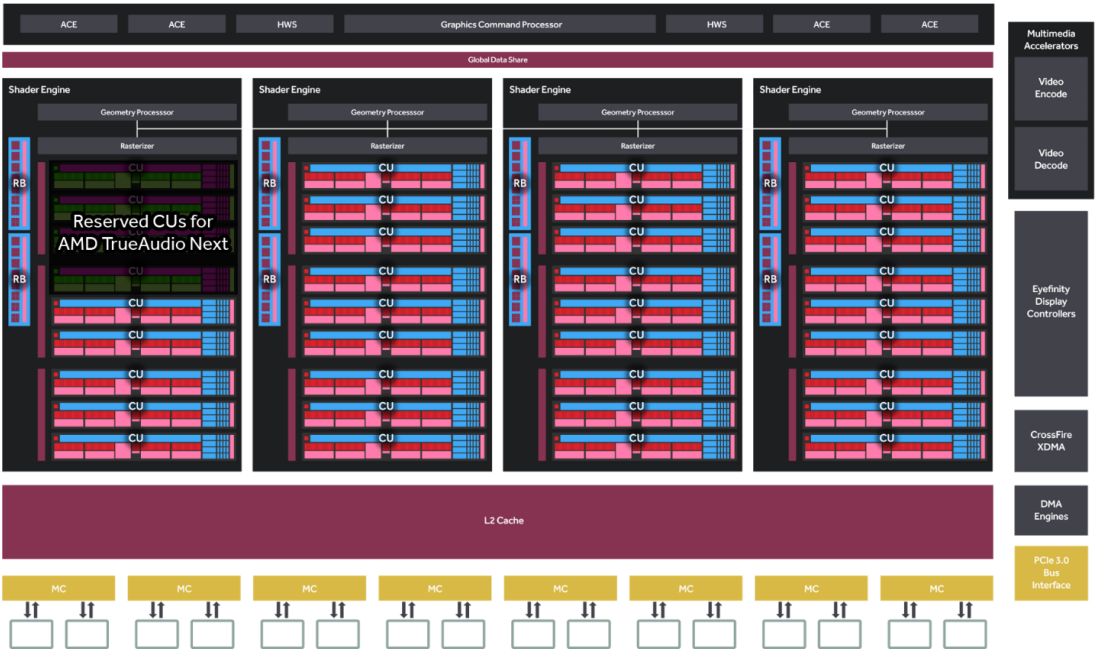
\includegraphics[width=.8\textwidth]{Figures/amd.png}
    \caption{Diagrama de bloque sobre arquitectura de chip Polaris 10}
    \label{fig:7}
\end{figure}

Además de las unidades estructurales presentes en ambas tarjetas, se deben tomar en cuenta que existen muchas otras características agregadas por cada compañía para solventar las necesidades de computo gráfico que existe en el nicho de venta, tales como unidades extra para el computo de teselado, texturas o iluminación con mejor rendimiento, una mayor ganancia a menor uso de voltaje, o soporte para diferentes APIs ligadas al rendimiento de aplicaciones, tales como DirectX o Vulkan~\cite{directx, vulkan}.
Presentando otro ejemplo, el \textit{whitepaper} de la arquitectura Polaris publicado por AMD menciona la capacidad de los controladores de las tarjetas gráficas de poder reservar unidades de procesamiento para tareas especificas, tales como procesado de audio.
Estas pueden ser oportunidades que permitan extender el dominio de la programación paralela en GPU, sin embargo, tomando en cuenta que solamente interesan aquellas propiedades que influyan directamente con la ejecución de códigos de programación paralela en GPU se omitirán por simplicidad. 
A continuación se presenta una tabla comparativa de las especificaciones de ambas tarjetas gráficas en torno a características generales, configuraciones de renderizado y rendimiento teórico sobre operaciones de punto flotante.

% Tabla V3
\renewcommand{\arraystretch}{1.5}
\begin{table}[ht!]
\centering
\caption{Comparación de especificaciones técnicas de tarjetas AMD RX570 y NVIDIA GTX960M.}
\begin{tabularx}{\textwidth}{XX|c|c|}
\cline{3-4}
                                                                    &                         & AMD RX570             & NVIDIA GTX960M        \\ \hline
\multicolumn{1}{|l|}{\multirow{2}{*}{Rendimiento Teórico}}          & FP32 (float)            & \(5.095\) {[}Tflop/s{]} & \(1.505\) {[}Tflop/s{]} \\ \cline{2-4} 
\multicolumn{1}{|l|}{}                                              & FP64 (double)           & \(318.5\) {[}Gflop/s{]} & \(47.04\) {[}Gflop/s{]} \\ \hline
\multicolumn{1}{|l|}{\multirow{3}{*}{Configuración de Renderizado}} & Unidades de Sombreado   & 2048 {[}SP{]}         & 640 {[}CU{]}          \\ \cline{2-4} 
\multicolumn{1}{|l|}{}                                              & Unidades de Texturizado & 128 {[}TMU{]}         & 40 {[}TMU{]}          \\ \cline{2-4} 
\multicolumn{1}{|l|}{}                                              & ROPs                    & 16 {[}ROP{]}          & 32c {[}ROP{]}         \\ \hline
\multicolumn{1}{|l|}{\multirow{3}{*}{Especificaciones Generales}}   & Clock Base              & 1168 {[}MHz{]}        & 1097 {[}MHz{]}        \\ \cline{2-4} 
\multicolumn{1}{|l|}{}                                              & Tamaño de Memoria       & 4 {[}GB{]}            & 8 {[}GB{]}            \\ \cline{2-4} 
\multicolumn{1}{|l|}{}                                              & Anchos de Banda         & \(224.0\)  {[}GB/s{]}   & \(80.19\) {[}GB/s{]}    \\ \hline
\end{tabularx}
\end{table}

\iffalse

%Tabla V2

\begin{table}[ht!]
\centering
\caption{Comparación de especificaciones técnicas de tarjetas AMD RX570 y NVIDIA GTX960M.}
\begin{tabular}{ll|c|c|}
\cline{3-4}
                                                                                             &                         & AMD RX570    & NVIDIA GTX960M \\ \hline
\multicolumn{1}{|l}{\begin{tabular}[c]{@{}l@{}}Rendimiento \\ Teorico\end{tabular}}          & FP32 (float)            & 5.095 TFLOPS & 1.505 TFLOPS   \\
\multicolumn{1}{|l}{}                                                                        & FP64 (double)           & 318.5 GFLOPS & 47.04 GFLOPS   \\ \hline
\multicolumn{1}{|l}{\begin{tabular}[c]{@{}l@{}}Configuración\\  de Renderizado\end{tabular}} & Unidades de Sombreado   & 2048 SP      & 640 CU         \\
\multicolumn{1}{|l}{}                                                                        & Unidades de Texturizado & 128 TMU      & 40 TMU         \\
\multicolumn{1}{|l}{}                                                                        & ROPs                    & 16 ROPs      & 32 ROPs        \\ \hline
\multicolumn{1}{|l}{General}                                                                 & Clock Base              & 1168 MHz     & 1097 MHz       \\
\multicolumn{1}{|l}{}                                                                        & Tamaño de Memoria       & 4 GB         & 4 GB           \\
\multicolumn{1}{|l}{}                                                                        & Ancho de Banda          & 224.0 GB/s   & 80.19 GB/s     \\ \hline
\end{tabular}
\end{table}



% Tabla V1

\begin{table}[h!]
\centering
\begin{tabular}{ll|c|c|}
\cline{3-4}
                                                  &                         & AMD RX570    & NVIDIA GTX960M \\ \hline
\multicolumn{1}{|l}{Rendimiento \newline Teórico}          & FP32 (float)            & 5.095 TFLOPS & 1.505 TFLOPS   \\
\multicolumn{1}{|l}{}                             & FP64 (double)           & 318.5 GFLOPS & 47.04 GFLOPS   \\ \hline 
\multicolumn{1}{|l}{Configuración de Renderizado} & Unidades de Sombreado   & 2048 SP      & 640 CU         \\
\multicolumn{1}{|l}{}                             & Unidades de Texturizado & 128 TMU      & 40 TMU         \\
\multicolumn{1}{|l}{}                             & ROPs                    & 16 ROPs      & 32 ROPs        \\ \hline
\multicolumn{1}{|l}{Características Generales}                      & Clock Base              & 1168 MHz     & 1097 MHz       \\
\multicolumn{1}{|l}{}                             & Tamaño de Memoria       & 4 GB         & 4 GB           \\
\multicolumn{1}{|l}{}                             & Ancho de Banda          & 224.0 GB/s   & 80.19 GB/s     \\ \hline
\end{tabular}
\caption{Comparación de especificaciones técnicas de tarjetas AMD RX570 y NVIDIA GTX960M}
\end{table}

\fi

\subsection{PROGRAMACIÓN EN ROCM Y COMPARATIVA A CUDA}

\hlabel{sec:3.2}

Antes de realizar cualquier tipo de acercamiento a la solución del problema propuesto, se deben mencionar algunos términos claves en el paradigma de programación paralela presente en las plataformas de desarrollo que se compararán, específicamente Instrucción Única y Múltiples Hilos (del inglés, \textit{Single Instruction Multiple Thread} o \textit{SIMT}).
El modelo \textit{SIMT} corresponde a una combinación del \textit{Multithreading} y \textit{Single Instruction Multiple Data}, una clasificación dentro de la Taxonomía de Flynn \cite{simt} de arquitectura de computadoras, la cual implica que una sola instrucción puede entregarse a distintas unidades de procesamiento para su ejecución simultanea.
Una serie de instrucciones ejecutadas es lo que se conoce como ``hilo'' o \textit{thread} y múltiples \textit{threads} que trabajan de forma paralela es lo que se llama como \textit{multithreading}.
Tomando en cuenta el modelo \textit{SIMT}, es que se trabaja con ambas plataformas de desarrollo (ROCm y CUDA), en las cuales cada una posee APIs representadas por métodos que facilitan la gestión de dispositivos (o tarjetas gráficas), eventos, tipos de memoria a utilizar (global o compartida), o librerías para trabajos específicos del área de HPC, presentados brevemente en el Capítulo~\hyperref[sec:1]{1}.

Dentro del dominio de la programación en CUDA y ROCm existe el termino ``kernel'', el cual corresponde a una encapsulación de instrucciones con forma de función la cual será enviada a la GPU con tal de ser ejecutada.
Parte de lo que se tiene que tomar en cuenta al momento de realizar programación paralela y por consecuencia en la definición de un kernel, son principalmente:

\begin{itemize}
    \item Condiciones de carrera, lo cual toma en cuenta que antes de comenzar con un nuevo conjunto de instrucciones (o kernel) todos los \textit{threads} comenzados con anterioridad deben terminar.
    \item Exclusión mutua, cuya idea es mantener la coherencia de datos al momento de usar recursos compartidos, o leer/escribir en memoria global.
\end{itemize}

\subsubsection{Suma de vectores}

Para poner un ejemplo, se podría pensar en la tarea de realizar una operación entre vectores, ya sea suma, producto interno o cualquier otro tipo de función \textit{element wise} o elemento a elemento.
En este caso no es necesario considerar las condiciones de carrera, pues la instrucción es una sola, sin embargo, lo que si hay que planear es el dominio de trabajo de cada \textit{thread}, por lo que si se utilizaran \(n\) \textit{threads} para realizar la suma de dos vectores de tamaño \(m\), cada \textit{thread} $i \in [ 0, n-1]$ tendría que trabajar netamente con los valores desde la posición $\left \lfloor{\frac{m}{n}}\right \rfloor  i$ hasta la posición $\left \lfloor{\frac{m}{n}}\right \rfloor i+1$.
Esto se puede esquematizar en el pseudo código del Algoritmo~\ref{alg:1}.
\begin{algorithm}
\caption{Kernel - Suma de vectores}
\label{alg:1}
\begin{algorithmic}[1]
\Procedure{VectorAdd}{vector1, vector2, vector3, m, n}
\State $i \leftarrow$ número de \textit{thread}
\State $j = \frac{m}{n} i$  
\For {j <  $\frac{m}{n} i + 1$}
    \State vector3[j] = vector1[j] + vectror2[j]
\EndFor
\EndProcedure
\end{algorithmic}
\end{algorithm}

Hasta hace algunos año una de las plataforma de HPC más utilizada era CUDA y es por esto que en posterior al lanzamiento de ROCm estuviera justificado la forma que tendría su forma de aplicación. 
Actualmente ROCm funciona en base al lenguaje C++ junto al dialecto \textit{Heterogeneous-Computing Interface for Portability} (HIP) el cual comprende una amplia gama de APIs para el aprovechamiento de los núcleos de procesamiento de tarjetas AMD, que a su vez poseen similitud en nombre y soporte para un sub conjunto de las funciones de CUDA.
Por estos motivos es que junto a HIP, ROCm presenta la herramienta Hipify, la cual corresponde a un programa que permite analizar gramaticalmente archivos de código de CUDA para generar código en C++ compilable por HIP.
Cabe destacar que existen dos variantes de este software, una en base al lenguaje Perl y otra en base al front end para compilaciones Clang, de los cuales se pueden obtener ventajas y desventajas de cada una. 
La principal ventaja de Hipify-Clang, es que al ser un traductor, realiza una revisión sintáctica de el o los archivos de entrada, lo cual indica en momento de ejecución si la traducción fue correcta o no. 
Esta misma característica de la versión en Clang es su mayor desventaja, pues si el código en CUDA C está incorrecto o fuera de los limites del software no se generará un programa en HIP.
Por otro lado, Hipify-Perl corresponde a una implementación en base a expresiones regulares, más directa en comparación a su contra parte, la cual siempre generará código de HIP independiente de su correctitud.
Además, una última desventaja de la versión de Perl es la falta de soporte a ciertas funciones de CUDA C \cite{HIP}.


Haciendo uso del ejemplo previo se presenta la Figura~\ref{fig:8}, la cual contiene la definición del kernel \textit{vectorAdd} como implementación del Algoritmo~\ref{alg:1}.
En este caso, se está considerando que al momento de ejecutar el kernel se hará con una configuración que genere un \textit{thread} por cada elemento del vector final en el que se almacenará la suma y debido a esto es que existe diferencia entre la linea 3-4 del Algoritmo~\ref{alg:1} y la condicional en la linea 7 del código de la Figura~\ref{fig:8}, además de los parámetros de entrada en cada uno.

\begin{figure}[h!]
\centering
\begin{lstlisting}[language=C, frame=single, breaklines=true, numbers=left, style=CudaStyle ]
__global__ void
vectorAdd(const float *A, const float *B, 
            float *C, int numElements)
{
    int i = blockDim.x * blockIdx.x + threadIdx.x;
    if (i < numElements)
    {
        C[i] = A[i] + B[i];
    }
}
\end{lstlisting}
\caption{Definición de kernel para suma de vectores.}
\label{fig:8}
\end{figure}

El código presentado en la Figura~\ref{fig:9} corresponde a una versión simplificada de la función principal {\verb main() } del archivo vectorAdd.cu presente en los ejemplos de la versión 11.2 del \textit{CUDA Toolkit} \cite{samples}.
La estructura en este corresponde a la siguiente:
\begin{itemize}
    \item \textbf{Lineas 5-10}: Configuración de tamaño de los 3 arreglos (representación de vectores) necesarios y su asignación de memoria respectiva.
    \item \textbf{Lineas 11-15}: Inicialización de ambos arreglos a sumar con números tipo \textit{float} aleatorios.
    \item \textbf{Lineas 16-23}: Definición de los 3 punteros a los arreglos necesarios en memoria de GPU, su asignación de memoria respectiva y la copia de datos desde memoria de CPU a GPU.
    \item \textbf{Lineas 25-27}: Calculo del número de \textit{threads} a utilizar en GPU y ejecución del kernel presentado en el Algoritmo~\ref{alg:1}. Para esta instancia en particular (pues el tamaño del arreglo esta asignado arbitrariamente a 5000), el número total de \textit{threads} será igual a $256\times \text{blocksPerGrid} = 256 \times (5000 + 256 - 1) \div 256 = 5255$ [\textit{thread}].
    \item \textbf{Lineas 29-36}: Copia de resultados del kernel al arreglo respectivo en CPU y liberación de memoria en CPU y GPU para evitar perdidas de memoria o \textit{memory leaks}.
\end{itemize}

En contraste con lo anterior, la Figura~\ref{fig:10} presenta la salida de ejecutar la herramienta \textit{Hipify} en su versión basada en Perl con el código de la Figura~\ref{fig:9} como entrada.
Haciendo énfasis en los cambios realizados por \textit{Hipify}, se deben destacar las lineas, (17, 18, 19), (22, 23, 27), 27 y (31, 32, 33) en las cuales se realizan asignaciones de memoria, se hacen transferencias de datos entre memoria de CPU y GPU, se ejecuta el kernel y se libera memoria, todo en GPU y tan solo cambiando la firma de los métodos utilizados por CUDA con su contra parte en HIP. 
El resultado de la ejecución de ambos kernel en tarjetas gráficas de AMD y NVIDIA para diversos tamaños de vectores se presentará en el Capítulo~\hyperref[sec:4]{4}.


\newpage

\begin{figure}[h!]
\centering
\begin{lstlisting}[language=C++, frame=single, breaklines=true,style=CudaStyle, basicstyle=\footnotesize, numbers=left]
#include <stdio.h>
#include <cuda_runtime.h>
int main(int argc, char* argv[])
{
    int numElements = 50000;
    size_t size = numElements * sizeof(float);
    
    float *h_A = (float *)malloc(size);
    float *h_B = (float *)malloc(size);
    float *h_C = (float *)malloc(size);
    for (int i = 0; i < numElements; ++i)
    {
        h_A[i] = rand()/(float)RAND_MAX;
        h_B[i] = rand()/(float)RAND_MAX;
    }
    float *d_A = NULL;
    cudaMalloc((void **)&d_A, size);
    float *d_B = NULL;
    cudaMalloc((void **)&d_B, size);
    float *d_C = NULL;
    cudaMalloc((void **)&d_C, size);
    cudaMemcpy(d_A, h_A, size, cudaMemcpyHostToDevice);
    cudaMemcpy(d_B, h_B, size, cudaMemcpyHostToDevice);

    int threadsPerBlock = 256;
    int blocksPerGrid =(numElements + threadsPerBlock - 1) / threadsPerBlock;
    vectorAdd<<<blocksPerGrid, threadsPerBlock>>>(d_A, d_B, d_C, numElements);

    cudaMemcpy(h_C, d_C, size, cudaMemcpyDeviceToHost);

    cudaFree(d_A);
    cudaFree(d_B);
    cudaFree(d_C);
    free(h_A);
    free(h_B);
    free(h_C);

    printf("Done\n");
    return 0;
}
\end{lstlisting}
\caption{Función main()  de un código CUDA para suma de vectores vectorAdd.cu.}
\label{fig:9}
\end{figure}

\newpage

\begin{figure}[h!]
\centering
\begin{lstlisting}[language=C++, frame=single, breaklines=true,basicstyle=\footnotesize, numbers=left, style=CudaStyle]
#include <stdio.h>
#include <hip/hip_runtime.h>
int main(int argc, char* argv[])
{
    int numElements = 50000;
    size_t size = numElements * sizeof(float);
   
    float *h_A = (float *)malloc(size);
    float *h_B = (float *)malloc(size);
    float *h_C = (float *)malloc(size);
    for (int i = 0; i < numElements; ++i)
    {
        h_A[i] = rand()/(float)RAND_MAX;
        h_B[i] = rand()/(float)RAND_MAX;
    }
    float *d_A = NULL;
    hipMalloc((void **)&d_A, size);
    float *d_B = NULL;
    hipMalloc((void **)&d_B, size);
    float *d_C = NULL;
    hipMalloc((void **)&d_C, size);
    hipMemcpy(d_A, h_A, size, hipMemcpyHostToDevice);
    hipMemcpy(d_B, h_B, size, hipMemcpyHostToDevice);

    int threadsPerBlock = 256;
    int blocksPerGrid =(numElements + threadsPerBlock - 1) / threadsPerBlock;
    hipLaunchKernelGGL(vectorAdd, dim3(blocksPerGrid), dim3(threadsPerBlock), 0, 0, d_A, d_B, d_C, numElements);
    hipMemcpy(h_C, d_C, size, hipMemcpyDeviceToHost);

    
    hipFree(d_A);
    hipFree(d_B);
    hipFree(d_C);
    free(h_A);
    free(h_B);
    free(h_C);

    printf("Done\n");
    return 0;
}
\end{lstlisting}
\caption{Función  main()  de un código compilable por HIP, resultado de la ejecución de la herramienta Hipify-Perl en el código de la Figura~\ref{fig:9}.}
\label{fig:10}
\end{figure}
\newpage

\subsubsection{Multiplicación de matrices}

Un marco referencial muy utilizado con tal de poder entender y así poner a prueba la programación paralela usando GPU es la multiplicación de matrices.
Considerando dos matrices $A, B \in \mathbb{R}^{n\times n}$, su multiplicación daría como resultado una matriz $C\in R^{n\times n}$ en la que el valor de cada coeficiente estaría dado por la formula,
\begin{equation*}
    c_{ij} = a_{i1}b_{1i} + a_{i2}b_{2i} + \dots + a_{in}b_{ni} = \sum_{k=1}^n a_{ik}b_{ki}
\end{equation*}
en donde $i, j \in [0,n]$ y \(a_{ij}\), \(b_{ij}\), \(c_{ij}\) corresponden a coeficientes de $A, B, C$ respectivamente.

En un principio, esto podría realizarse de forma secuencial y de manera exhaustiva realizando productos internos (ver Figura~\ref{fig:11}) entre la combinatoria de todas las filas y columnas de las matrices \(A\) y \(B\).

\begin{figure}[h!]
\centering
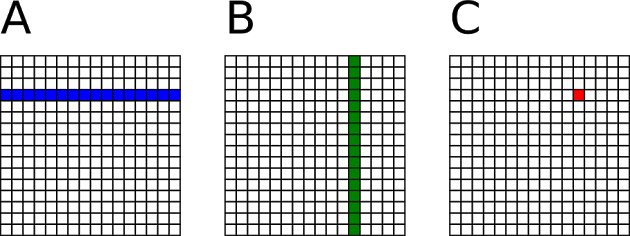
\includegraphics[width=0.8\textwidth]{Figures/naive.png}
\caption{Esquema de procedimiento común en una multiplicación de matrices con implementación secuencial, fuente:~\cite{matrixM}.}
\label{fig:11}
\end{figure}

Ahora, haciendo uso de una implementación en programación paralela y la ejecución en una GPU, se podría replicar lo propuesto a la hora de realizar la suma de dos vectores en la sección anterior, asignando a cada \textit{thread} la tarea de realizar uno de los productos internos, por lo que el total de \textit{threads} tendría que ser igual o mayor al número de elementos de la matriz resultante \(C\).
Esto se puede esquematizar en la definición de la función {\verb main() } y kernel propuestos en los Algoritmo~\ref{alg:2},\ref{alg:3}.

\begin{algorithm}
\caption{Función main()  - Multiplicación de matrices}
\label{alg:2}
\begin{algorithmic}[1]
%\algsetup{linenosize=<size>}
\Procedure{main}{}
\State definir A, B, C en la memoria de CPU
\State inicializar A, B
\State definir Agpu, Bgpu, Cgpu en la memoria de GPU
\State copiar memoria de A a Agpu
\State copiar memoria de B a Bgpu
\State definir cantidad de \textit{threads} en \(i\)
\State matrixMul<<i>>(Agpu, Bgpu, Cgpu)
\State copiar memoria de Cgpu a C
\EndProcedure
\end{algorithmic}
\end{algorithm}

\begin{algorithm}
\caption{Kernel - Multiplicación de matrices}
\label{alg:3}
\begin{algorithmic}[1]
%\algsetup{linenosize=<size>}
\Procedure{matrixMul}{Agpu, Bgpu, Cgpu}
\State definir tmp
\State calcular fila y columna de Cgpu en la que se trabajará (i,j)
\For {k = [0,n-1]}
    \State tmp = tmp + Agpu(k, j)*Bgpu(i, k)
\EndFor
\State Cgpu(i,j) = tmp
\EndProcedure
\end{algorithmic}
\end{algorithm}

Antes de continuar con las siguientes optimizaciones posibles para un algoritmo de multiplicación de matrices, se debe hacer la distinción entre lo que implica el uso de memoria global y memoria compartida.
La memoria global corresponde a registro accesibles por todas las unidades de procesamiento presentes en una GPU, mientras que la memoria compartida hace referencia a aquella que se puede acceder y es ``visible'' por \textit{threads} de un mismo bloque.
En este contexto, bloque hace referencia a la jerarquía de generación de threads de CUDA C y HIP, partiendo por una grilla, compuesta por bloques y que a su vez esta compuesta por cierta cantidad de \textit{threads}.
Estas abstracciones son partes de los parámetros presentes al momento de ejecutar un kernel, los cuales definen la cantidad total de \textit{threads}.

Para evitar limitaciones en el rendimiento de este algoritmo (más conocido como cuello de botella o \textit{bottle neck}) es que se le puede realizar una optimización utilizando \textit{Tiling}, o la división de la matriz final en bloques de tamaño arbitrario con tal de transferir la información de las matrices a las que se debe acceder a memoria compartida por \textit{threads} de un mismo grupo de trabajo, la cual se caracteriza por ser de acceso mucho más rápido.

Si bien con esto se pierde un poco de tiempo haciendo la transferencia de datos, la recompensa es mucho mayor por el acceso directo a los elementos de las matrices \(A\) y \(B\) a la hora de calcular los productos punto.
En este nuevo esquema y en las siguientes optimizaciones que se presentarán, el único cambio se encuentra en el código del kernel, por lo cual solo se realizarán actualizaciones del mismo.
En el pseudo código del Algoritmo~\ref{alg:4} sintetiza lo planteado, en donde, si se toma como ejemplo el diagrama de la Figura~\ref{fig:12}, se entiende que para ese caso la cantidad de \textit{Tiles} es igual a 2.
Así, en el primer ciclo for de la linea 6 del Algoritmo~\ref{alg:4}, cada thread encargado de generar \(C_{0,0}\) trabajará en trasladar a memoria compartida los elementos de la sub matriz \(A_{0,0}\) y \(B_{0,0}\) para generar una respuesta parcial y sincronizar, cosa que corresponde a generar una barrera que espera a que todos los \textit{threads} terminen sus instrucciones.
Luego, en la segunda iteración (y final para este caso), el grupo de \textit{threads} encargados de calcular \(C_{0,0}\) cargarán en memoria compartida \(A_{0,1}\) y \(B_{1,0}\), para obtener el resultado completo.


\begin{algorithm}
\caption{Kernel - Multiplicación de matrices}
\label{alg:4}
\begin{algorithmic}[1]
%\algsetup{linenosize=<size>}
\Procedure{matrixMul}{Agpu, Bgpu, Cgpu}
\State definir tamañoTile
\State definir A\_tile, B\_tile en memoria compartida
\State calcular fila y columna de Cgpu en la que se trabajará (i,j)
\State definir tmp
\For {tileIdx = [0, $n \div $tamañoTile]}
    \State calcular fila y columna de A\_Tile/B\_Tile en la que se trabajará (a,b)
    \State asignar valor correspondiente desde Agpu a A\_Tile 
    \State asignar valor correspondiente desde Bgpu a B\_Tile 
    \State sincronizar \textit{threads}
    \For {k = [0, tamañoTile]}
        \State tmp = tmp + A\_Tile(k, b) + B\_Tile(a, k)
    \EndFor
    \State sincronizar \textit{threads}
\EndFor
\State Cgpu(i,j) = tmp
\EndProcedure
\end{algorithmic}
\end{algorithm}

\begin{figure}[h!]
\centering
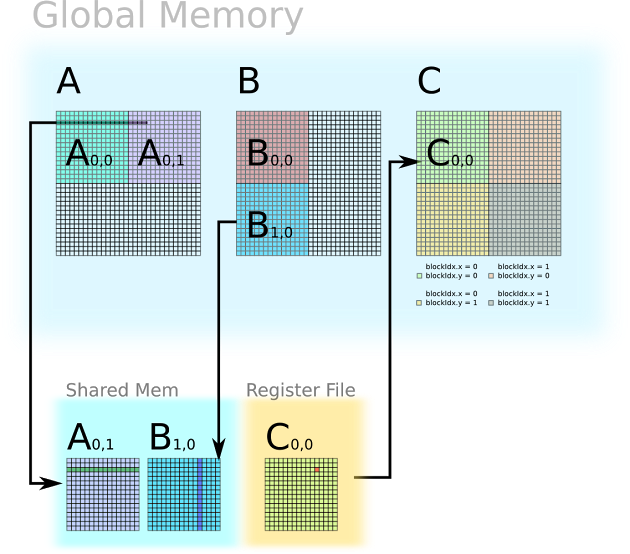
\includegraphics[width=0.8\textwidth]{Figures/opt1.png}
\caption{Esquema de implementación paralela para multiplicación de matrices usando \textit{Tiling}, fuente:~\cite{matrixM}.}
\label{fig:12}
\end{figure}

La coalescencia de memoria o \textit{memory coalescing} corresponde a un termino de la programación paralela en GPU la cual se refiere a un acceso ordenado a los segmentos de memoria que posee la tarjeta con la que se trabaja.
Esto ocurre, pues cada vez que se realiza un acceso a memoria por parte de un \textit{warp} o wavefront (conjunto de \textit{threads}), este debe ser respecto a un bloque de memoria contiguo.
Por tanto, si en una instrucción se debe acceder a celdas de memorias que se encuentran en sectores lejanos, el número de accesos es mayor y en consecuencia, más costoso computacionalmente.

Así, una solución para este problema es trasponer la matriz B al momento de trasladar los datos desde memoria global a memoria compartida, lo cual se puede implementar como un cambio en la linea 9 y 12 del Algoritmo~\ref{alg:5} respecto del Algoritmo~\ref{alg:4}. 

\begin{algorithm}
\caption{Kernel - Multiplicación de matrices con \textit{memory coalescing}}
\label{alg:5}
\begin{algorithmic}[1]
%\algsetup{linenosize=<size>}
\Procedure{matrixMul}{Agpu, Bgpu, Cgpu}
\State definir tamañoTile
\State definir A\_tile, B\_tile en memoria compartida
\State calcular fila y columna de Cgpu en la que se trabajará (i,j)
\State definir tmp
\For {tileIdx = [0, $n \div $tamañoTile]}
    \State calcular fila y columna de A\_Tile/B\_Tile en la que se trabajará (a,b)
    \State asignar valor correspondiente desde Agpu a A\_Tile 
    \State asignar valor correspondiente desde Bgpu a B\_Tile // de forma traspuesta 
    \State sincronizar \textit{threads}
    \For {k = [0, tamañoTile]}
        \State tmp = tmp + A\_Tile(k, b) + B\_Tile(k, a)
    \EndFor
    \State sincronizar \textit{threads}
\EndFor
\State Cgpu(i,j) = tmp
\EndProcedure
\end{algorithmic}
\end{algorithm}

Finalmente, sumado a las variantes de código explicadas, se puede analizar la cantidad de operaciones de bajo nivel que se designan al momento de compilar el archivo binario. 
En la arquitectura de unidades de procesamiento (al menos la presente en Maxwell) solo se permite realizar un operando entre elementos almacenados en la memoria compartida, lo cual se contra resta con el producto interno, el cual necesita una suma y una multiplicación en cada iteración del arreglo en memoria compartida (linea 12 del Algoritmo~\ref{alg:5}).
Esto podría ser solucionado utilizando memoria global para alguna de las dos matrices, pero con esta medida se perdería parte del trabajo realizado por el \textit{Tiling} en la primera variante.
Entonces, una alternativa viable es utilizar el producto externo en vez del producto interno.
Este se define a partir de la formula,

\begin{equation*}
u \otimes v = 
\begin{bmatrix} 
	u_1v_1 & u_1v_2 & \dots & u_1v_n\\
	u_2v_1 & u_2v_2 & \dots & u_2v_n\\
	\vdots & \vdots & \ddots & \vdots \\
	u_mv_1 & u_mv_2 & \dots & u_mv_n\\
	\end{bmatrix}
\end{equation*}



en donde $u\in R^m$ y $v\in R^n$.
De acuerdo a esta definición, por consecuencia la multiplicación de dos matrices \(A\) y \(B\) esta definida por,
\begin{equation*}
    C = A\,B = \sum_{i=1}^n a_i \otimes b^T_i
\end{equation*}
en la cual \(a_i\) es la i-esima columna de \(A\) y $b_i^T$ es la i-esima fila de \(B\).

Para poder aplicar el producto externo junto al \textit{Tiling}, se debe implementar el traspaso de datos de tan solo la matriz \(A\) a la memoria compartida del tamaño de un \textit{Tile} y realizar la operatoria con toda una fila de \(B\), como se ejemplifica en la Figura~\ref{fig:13}.

\begin{figure}[h!]
\centering
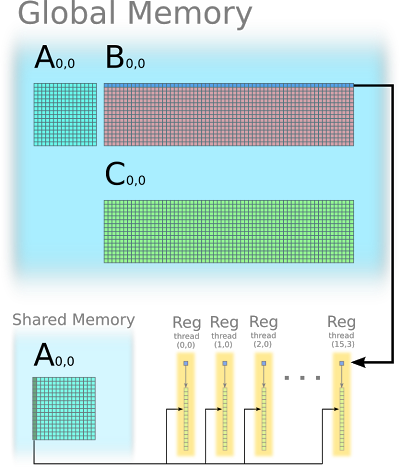
\includegraphics[width=0.8\textwidth]{Figures/opt2.png}
\caption{Esquema de implementación paralela para multiplicación de matrices usando \textit{Tiling} y el producto externo, fuente:~\cite{matrixM}.}
\label{fig:13}
\end{figure}

En el Algoritmo~\ref{alg:6}, se incluye el pseudo código de lo que sería una implementación de multiplicación de matrices aplicando todas las mejoras revisadas, además de aquellas que sirven para mejorar la optimización por compilación, tales como pre obtención de vectores y desenrollado explicito de ciclos.
Respecto al Algoritmo~\ref{alg:6}, se debe recalcar que a pesar de que tanto matrices \(B\) como \(C\) se accedan desde memoria global, no es necesario realizar ninguna trasposición para evitar un acceso no coalescente ya que en la última implementación ya se esta considerando un acceso por fila o \textit{row major}.

\begin{algorithm}
\caption{Kernel - Multiplicación de matrices utilizando producto externo y \textit{Tiling}.}
\label{alg:6}
\begin{algorithmic}[1]
%\algsetup{linenosize=<size>}
\Procedure{matrixMul}{Agpu, Bgpu, Cgpu}
\State definir tamañoTile
\State definir A\_tile, A\_tile2 en memoria compartida
\State obtener y asignar un tile de Agpu en A\_tile
\State sincronizar \textit{threads}
\For {tileIdx = [0, $n \div $tamañoTile]}
    \State obtener y asignar un tile siguiente de Agpu en A\_tile2
    \State calcular C utilizando A\_tile
    \State sincronizar \textit{threads}
    \State intercambiar punteros entre A\_tile y A\_tile2
\EndFor
\State guardar tile correspondiente en la memoria global de C
\EndProcedure
\end{algorithmic}
\end{algorithm}

Los resultados y el análisis de los mismo respecto al rendimiento de las tarjetas gráficas NVIDIA GTX960M y AMD RX570 en los diferentes algoritmos de suma de vectores y multiplicación de matrices se presentarán en el Capítulo~\hyperref[sec:4]{4}. 

\subsection{MÉTODO DE LATTICE BOLTZMANN}

El método de Lattice Boltzmann corresponde a una forma de realizar simulación de dinámica de fluidos a partir de una resolución directa de las ecuaciones de Navier-Stokes, sistema que define el comportamiento de líquidos viscosos procurando la conservación de masa y momentum~\cite{paperB}. 
Esto se logra a partir de las \textit{Shallow Water Equations} (del inglés ecuaciones de agua poco profunda), las cuales corresponden a un sistema de ecuaciones diferenciales parciales obtenidas a través de la integración vertical de las ecuaciones de Navier-Stokes y por ende más simples en terminos computacionales. Las SWE describen la evolución de la superficie libre de los fluidos a los que se aplican y corresponden a las siguientes ecuaciones

\begin{align}
    & \frac{\delta h}{\delta t} + \frac{\delta(hu)}{\delta x} + \frac{\delta(hv)}{\delta y} = 0 \\
    & \frac{\delta(hu)}{\delta t} + \frac{\delta}{\delta t} \left( hu^2 + \frac{1}{2}gh^2 \right) + \frac{\delta(huv)}{\delta y} = -gh\frac{\delta b}{\delta x} + F_1 \\
    & \frac{\delta(hv)}{\delta t} + \frac{\delta(huv)}{\delta x} + \frac{\delta}{\delta y}\left( hu^2 + \frac{1}{2}gh^2 \right) = -gh\frac{\delta b}{\delta y} + F_2
\end{align}


donde \(x\) e \(y\) conforman una posición cartesiana, \(t\) es el tiempo, \(h(x,y)\) es la altura del fluido, \(u(x,y,t)\) y \(v(x,y,t)\) son las componentes de velocidades en \(x\) e \(y\) respectivamente, \(b(x,y)\) es la elevación batimétrica, \(g\) es la constante gravitacional, y $F = (F_1, F_2)$ es la fuerza en términos de la dirección \(i\). 
La ecuación \((1)\) describe la conservación de la masa, y las ecuaciones \((2)\) y \((3)\) describen la conservación de momento \cite{paperB}.

El LBM ocupa una meso escala, termino intermedio entre una macro escala,la cual considera volúmenes de partículas como unidad de medida, y una micro escala, la cual trabaja con unidades atómicas. 
El método utiliza \textit{lattice units} (\textit{lu}) como unidades de distancia, \textit{time step} (\textit{ts}) como unidades de tiempo y una malla \(D2Q9\) (2 dimensiones y 9 velocidades discretas) por cada ``particula'' observada (ver Figura~\ref{fig:14}). 
La malla mencionada, se comprende de velocidades que están descritas de la siguiente manera:
\begin{align*}
    e_\alpha = 
     \begin{cases}
       (0,0) & \alpha = 0,\\
       e \left(\cos\frac{(\alpha - 1)\pi}{4}, \sin\frac{(\alpha - 1)\pi}{4} \right) & \alpha = 1, 2, 3, 4, \\
       \sqrt{2} e \left(\cos\frac{(\alpha - 1)\pi}{4}, \sin\frac{(\alpha - 1)\pi}{4} \right) & \alpha = 5, 6, 7, 8,\\
     \end{cases}
\end{align*}  
\begin{figure}
    \centering
    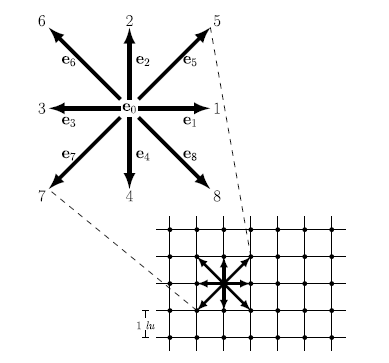
\includegraphics[scale=0.7]{Figures/d2q9.png}
    \caption{Malla D2Q9}
    \label{fig:14}
\end{figure}
donde $e = $ \textit{lu}\(/\)\textit{ts}. 
Usando el operador Bhatnagar–Gross–Krook para las colisiones del sistema, la ecuación del método queda de la siguiente forma \cite{bgk}:

\begin{align}
    f_\alpha(x + e_\alpha\Delta t, t + \Delta t) - f_\alpha(x,t) = -\frac{1}{\tau}[f_\alpha(x,t) - f^{(eq)}(x,t)] + S_\alpha(x,t)
\end{align}

donde $x = (x, y)$, \(\tau\) es el tiempo de relajación, \(f_\alpha\) es la función de distribución, $f_\alpha^{(eq)}$ es la función de distribución de equilibrio y \(S_\alpha(x,t)\) representa el termino de fuente, el cual se define de la siguiente manera:

\begin{align}
    S_\alpha = 
     \begin{cases}
       0 & \alpha = 0\\
       \dfrac{\Delta t}{6e^2}e_{\alpha i}F_i(x,t) - w_\alpha\dfrac{g\overline{h}(x,t)}{e^2}[b(x + e_\alpha\Delta t) - b(x)], & \alpha = 1,\dots,8 \\
     \end{cases}
\end{align} 

el cual incluye diferentes términos en su definición, tales como fuerzas superficiales, fuerzas volumétricas y el efecto \textit{bed slope}. 

A partir de la formula (5) y los aspectos mencionados en el Capítulo~\hyperref[sec:3.2]{3.2} es que se debe implementar LBM para programación paralela en GPU, principalmente pensando en el diseño de los elementos de las funciones de distribución (9 por cada ``nodo'') y que para poder calcular cada macro componente (fuerzas en cada eje y altura de la superficie del liquido) se necesitan elementos de las fuerzas de nodos adyacentes, por lo que se necesitaría una gestión adecuada de recursos en memoria.

Para la posterior experimentación, se utilizarán dos códigos generados por Álvaro Salinas, M.Sc., para su tesis titulada \textit{A high performance GPU implementation of the Lattice Boltzmann Method with open boundary conditions for solving the Shallow Water Equations in real scenarios}, cuya redacción fue para optar al grado de magíster en ciencias de la ingeniería informática en la Universidad Técnica Federico Santa María \cite{thesisB}.
Las implementaciones fueron, un framework general para futuros trabajos con distintas aplicaciones y funciones de equilibrio posibles, y una versión optimizada para la aplicación de las \textit{Shallow Water Equations} y condiciones de borde trabajadas en el paper \textit{Well-balanced open boundary condition in a lattice Boltzmann model for shallow water with arbitrary bathymetry} \cite{paperB}. 

Con tal de evitar cualquier tipo de error es que se planteó para ambas un \textit{Pull Scheme}, el cual consiste en utilizar 2 arreglos de memoria global en GPU para almacenar los 9 elementos de distribución de fuerzas de cada nodo con tal de reservar uno para lectura y otro para escritura respectivamente en cada \textit{time step}.
También, el diseño de estos se esquematiza de tal manera que exista un acceso coalescente a los arreglos, lo cual se logra posicionando de forma contigua aquellos elementos que se necesitan en una misma sección del kernel.
Esto fue nombrado como \textit{Struct of Arrays (SoA)} o arreglo de estructuras, mientras que una diseño no coalescente sería una estructura de arreglos o \textit{Array of Structs (AoS)} (ver Figura~\ref{fig:15}).

\begin{figure}[h!]
\centering
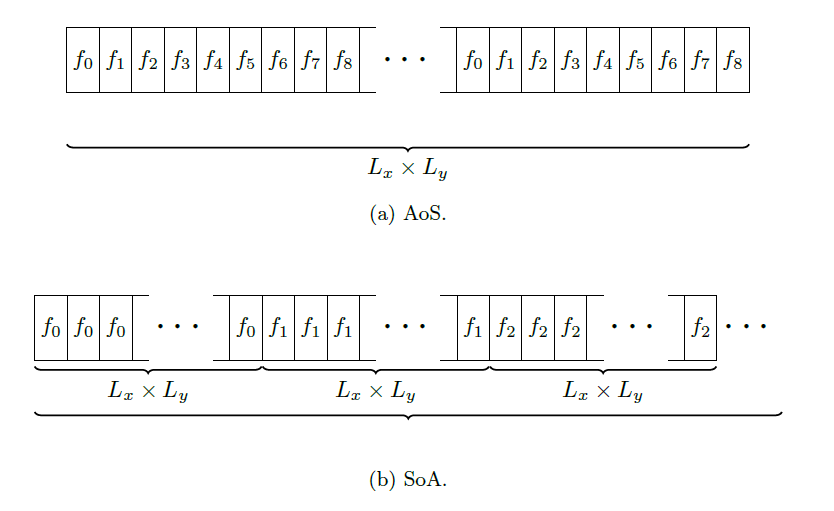
\includegraphics[width=0.6\textwidth]{Figures/layouts.png}
\caption{Diagrama de una Estructura de Arreglos \textit{(SoA)} y un Arreglo de Estructuras \textit{(AoS)}, fuente: \cite{thesisB}.}
\label{fig:15}
\end{figure}

\newpage


Para conseguir nuevos resultados y contrastar con los experimentos a realizar sobre los códigos de multiplicación de matrices, es que de todas formas se ejecutará una variación del código original del \textit{framework} con tal de no utilizar un acceso coalescente a la memoria y así analizar su efecto tanto en el tiempo de computo general como por cada sección del kernel de \textit{Pull Scheme}, cuya estructura general se presenta en el Algoritmo~\ref{alg:7}.

\begin{algorithm}
\caption{Kernel - \textit{Pull Scheme} en LBM}
\label{alg:7}
\begin{algorithmic}[1]
%\algsetup{linenosize=<size>}
\Procedure{TimeStep}{} %\(f_1\), \(f_2\), \(h\), \(b\), \(e\), \(Lx\), \(Ly\)
\If{se trabaja dentro del dominio de tamaño $Lx\times Ly$}
    \State definir \(f_\text{local}\)
    \For{fuerza $\alpha = [0,8]$}
        \If{necesita condición de borde abierta}
            \State \(f_\text{local}[\alpha]\) = \(f1[\alpha]\)
        \Else
            \State calcular S(\(\alpha\), \(h\), \(b\), \(e\))
            \State \(f_\text{local}[\alpha]\) = \(f1[\text{vecindario}][\alpha]\) + S
        \EndIf
    \EndFor
    \For{fuerza $\alpha = [0,8]$}
        \If{necesita condición de rebote \textit{Bounce Back}}
            \If{$\alpha \in {1,3,5,7}$}
                \State \(f_\text{local}[\alpha]\) = $f_\text{local}[\alpha + 2]$
            \Else
                \State \(f_\text{local}[\alpha]\) = $f_\text{local}[\alpha - 2]$
            \EndIf
        \EndIf
    \EndFor
    \State calcular variables macroscópicas \(h\), \(u\), \(v\)
    \For{fuerza $\alpha = [0,8]$}
        \State recalcular $f^{(eq)}$ = EDF(\(\alpha\), \(h\), \(u\), \(v\), \(e\))
        \State calcular y definir \(f_2[\alpha]\)
    \EndFor
\EndIf
\EndProcedure
\end{algorithmic}
\end{algorithm}

Con tal de obtener dicha comparativa, el código del kernel principal de \textit{LBM Framework} se subdividirá en los siguientes 3 kernels:

\begin{itemize}
    \item \verb|sourceForcing()|, en el que se hará el calculo parcial de las componentes de la función de distribución \(f_\alpha\) y aplicarán las condiciones de borden configuradas. Lineas 3 a 15 del Algoritmo~\ref{alg:7}.
    \item \verb|varMacroscopica|, en donde se recalcularán las variables macroscopicas. Linea 16 del Algoritmo~\ref{alg:7}.
    \item \verb|fUpdate()|, en el que se recalcularán los elementos de la función de equilibrio para el \textit{time step} actual y se recalculará \(f\). Linea 17 del Algoritmo~\ref{alg:7}.
\end{itemize}